% Harus dimuat terlebih dahulu, digunakan agar file PDF memiliki format karakter yang benar.
% Untuk informasi lebih lanjut, lihat https://ctan.org/pkg/cmap.
\RequirePackage{cmap}

% Format dokumen sebagai paper konferensi menggunakan aturan IEEEtran terbaru (v1.8b).
% Untuk informasi lebih lanjut, lihat http://www.michaelshell.org/tex/ieeetran/.
\documentclass[a4paper, conference]{IEEEtran}

% Format encoding font dan input menjadi 8-bit UTF-8.
\usepackage[T1]{fontenc}
\usepackage[utf8]{inputenc}
\usepackage{amsmath}

% Digunakan untuk mengatur margin dokumen.
\usepackage{textcomp}

% Format bahasa menjadi bahasa indonesia dan inggris.
\usepackage[indonesian]{babel}

% Digunakan untuk tujuan demonstrasi.
\usepackage{mwe}

% Digunakan untuk menampilkan font dengan style yang lebih baik.
\usepackage[zerostyle=b,scaled=.75]{newtxtt}

% Digunakan untuk menampilkan tabel dengan style yang lebih baik.
\usepackage{booktabs}
\usepackage[table,xcdraw]{xcolor}
% Digunakan untuk menampilkan gambar pada dokumen.
\usepackage{graphicx}

% Digunakan untuk menampilkan potongan kode.
\usepackage{listings}
\lstset{
  basicstyle=\ttfamily,
  columns=fixed,
  basewidth=.5em,
  xleftmargin=0.5cm,
  captionpos=b
}

\usepackage{tabularx}
\usepackage{wrapfig}
% Digunakan agar backticks (`) dapat dirender pada PDF.
% Untuk informasi lebih lanjut, lihat https://tex.stackexchange.com/a/341057/9075.
\usepackage{upquote}

% Digunakan untuk menyeimbangkan bagian akhir dokumen dengan dua kolom.
\usepackage{balance}

% Kapitalisasi caption tabel
\usepackage{caption}
\captionsetup[table]{
    justification=centering, % Memusatkan caption
    labelsep=newline, % Memisahkan label "TABLE 1" dengan judul dengan baris baru
    textfont={sc}, % Membuat teks menjadi kapital
    labelfont={sc} % Membuat teks menjadi kapital
}


% Digunakan untuk menampilkan pustaka.
\usepackage[square,comma,numbers,sort&compress]{natbib}

% Mengubah format ukuran teks pada natbib.
\renewcommand{\bibfont}{\normalfont\footnotesize}

% Jika melebihi 3 penulis dapat dilakukan linebreakend 
\makeatletter
\newcommand{\linebreakand}{%
  \end{@IEEEauthorhalign}
  \hfill\mbox{}\par
  \mbox{}\hfill\begin{@IEEEauthorhalign}
}
\makeatother

% Menambah nama penulis ketika menggunakan perintah \citet.
% Untuk informasi lebih lanjut, lihat https://tex.stackexchange.com/a/76075/9075.
\usepackage{etoolbox}
\makeatletter
\patchcmd{\NAT@test}{\else \NAT@nm}{\else \NAT@hyper@{\NAT@nm}}{}{}
\makeatother

% Digunakan untuk melakukan linewrap pada pustaka dengan url yang panjang
% jika terdapat hyphens
\usepackage[hyphens]{url}

% Digunakan untuk menambah hyperlink pada referensi.
\usepackage{hyperref}

% Menonaktifkan warna dan bookmark pada hyperref.
\hypersetup{hidelinks,
  colorlinks=true,
  allcolors=black,
  pdfstartview=Fit,
  breaklinks=true
}

% Digunakan untuk membenarkan hyperref pada gambar.
\usepackage[all]{hypcap}

% Digunakan untuk menampilkan beberapa gambar
%\usepackage[caption=false,font=footnotesize]{subfig}
\usepackage{multirow}
\usepackage{longtable}
\usepackage{graphicx}
\usepackage{subcaption}
\usepackage{stfloats}
\usepackage{float}
% nama
\newcommand{\name}{Aldi Fahmi Sihotang}
\newcommand{\authorname}{Sihotang, Aldi Fahmi}
\newcommand{\nickname}{Aldi}
\newcommand{\advisor}{Dr. Eko Mulyanto Yuniarno, S.T., M.T.}
\newcommand{\coadvisor}{Dr. Supeno Mardi Susiki Nugroho,S.T.,M.T.}

% identitas
\newcommand{\nrp}{0721 18 4000 0039}
\newcommand{\advisornip}{19680601 199512 1 009}
\newcommand{\coadvisornip}{19700313199512 1 001}
\newcommand{\email}{07211840000039@student.its.ac.id}
\newcommand{\advisoremail}{ekomulyanto@ee.its.ac.id}
\newcommand{\coadvisoremail}{mardi@its.ac.id}

% judul
\newcommand{\tatitle}{PENGEMBANGAN KURSI RODA OTONOM UNTUK MENGIKUTI MANUSIA BERBASIS \emph{YOLOv11}}
\newcommand{\engtatitle}{YOLOv11-BASED AUTONOMOUS WHEELCHAIR DEVELOPMENT FOR FOLLOWING HUMAN}
% tempat
\newcommand{\place}{Surabaya}   

% jurusan
\newcommand{\studyprogram}{Teknik Komputer}
\newcommand{\engstudyprogram}{Computer Engineering}

% fakultas
\newcommand{\faculty}{Teknologi Elektro dan Informatika Cerdas}
\newcommand{\engfaculty}{Intelligence Electrical and Informatics Technology}

% singkatan fakultas
\newcommand{\facultyshort}{FTEIC}
\newcommand{\engfacultyshort}{ELECTICS}

% departemen
\newcommand{\department}{Teknik Komputer}
\newcommand{\engdepartment}{Computer Engineering}

% Tambahkan format tanda hubung yang benar di sini
\hyphenation{
  ro-ket
  me-ngem-bang-kan
  per-hi-tu-ngan
}


\begin{document}

% Ubah kalimat berikut sesuai dengan judul penelitian.
\title{\engtatitle{}}

% Ubah kalimat-kalimat berikut sesuai dengan nama, institusi, alamat dan kontak penulis.
\author{
  \IEEEauthorblockN{1\textsuperscript{st} \advisor{}}
  \IEEEauthorblockA{\textit{dept. of \engstudyprogram{}}\\
    \textit{Institut Teknologi Sepuluh Nopember}\\
    Surabaya, Indonesia 60111\\
    \email{}}

  \and
  \IEEEauthorblockN{2\textsuperscript{nd} \coadvisor{}}
  \IEEEauthorblockA{\textit{dept. of \engstudyprogram{}}\\
    \textit{Institut Teknologi Sepuluh Nopember}\\
    Surabaya, Indonesia 60111\\
    \advisoremail{}}

  \and
  \IEEEauthorblockN{3\textsuperscript{rd} \name{}}
  \IEEEauthorblockA{\centerline{\textit{dept. of \engstudyprogram{}}}\\
    \textit{Institut Teknologi Sepuluh Nopember}\\
    Surabaya, Indonesia 60111\\
    \coadvisoremail{}}
}

% Digunakan untuk menampilkan judul dan deskripsi penulis.
\maketitle
% Mengubah keterangan `Abstract` ke bahasa indonesia.
% Hapus bagian ini untuk mengembalikan ke format awal.
% \renewcommand\abstractname{Abstrak}

\begin{abstract}

  % Ubah paragraf berikut sesuai dengan abstrak dari penelitian.
  This study aims to develop an autonomous wheelchair control system that can follow human movement in real-time. This system integrates the object detection algorithm \emph{YOLOv11} and body motion tracking using MediaPipe Pose, utilizing the optimal viewing angle as the basis for visual data collection. The camera is placed on the user's glasses to obtain the optimal viewing angle in detecting and tracking user movement. This system is designed to operate wirelessly using the ESP32 module, providing flexibility and efficiency in controlling wheelchair movement. Testing was conducted in a controlled environment to ensure the accuracy and speed of user movement detection and tracking. The results showed that the system can follow user movement accurately and responsively, making a significant contribution to the development of smarter and more independent health mobility technology.


\end{abstract}

% Mengubah keterangan `Index terms` ke bahasa indonesia.
% Hapus bagian ini untuk mengembalikan ke format awal.
% \renewcommand\IEEEkeywordsname{Kata kunci}

\begin{IEEEkeywords}

  % Ubah kata-kata berikut sesuai dengan kata kunci dari penelitian.
  Autonomous Wheelchair, YOLOv11, MediaPipe Pose, Optimal Viewing Angle, Motion Detection, Wireless Control, Health Mobility.

\end{IEEEkeywords}


% Ubah bagian berikut sesuai dengan konten-konten yang akan dimasukkan pada dokumen
% Ubah judul dan label berikut sesuai dengan yang diinginkan.
\section{Introduction}
\label{sec:introduction}

% Ubah paragraf-paragraf pada bagian ini sesuai dengan yang diinginkan.

The integration of \emph{Internet of Things (IoT)} and \emph{deep learning} technologies is increasingly adopted in the development of autonomous control systems, particularly for healthcare and mobility applications. An autonomous wheelchair is one solution that can improve the quality of life for people with disabilities by providing independence in movement. One of the key technologies that can support the development of an autonomous wheelchair is the \emph{ESP32} module. According to research conducted by \emph{Ekatama} (2024), the \emph{ESP32} can control devices wirelessly using \emph{Wi-Fi} and \emph{Bluetooth} connectivity, offering greater flexibility in controlling the wheelchair. The use of this module allows users to effectively control the wheelchair without relying on limited manual control \cite{ekatama2024perancangan}.

In addition to wireless control aspects, an autonomous system that follows the user's movements requires technology capable of detecting body movements in real-time. Research by \emph{Wijaya et al.} (2022) has demonstrated the reliability of the \emph{YOLO V3} algorithm in detecting objects quickly and accurately, which can be used to track human movements. However, in this study, the \emph{YOLOv11} algorithm, the latest version of \emph{YOLO}, is integrated with \emph{MediaPipe Pose}, a framework that can detect and track human body positions. The combination of these two technologies allows the system to accurately follow the user's movements based on the optimal viewpoint obtained from a camera mounted on the user's glasses. With this approach, the wheelchair can naturally follow the user's movements, supporting higher autonomy \cite{wijaya2022deteksi}.

The autonomous wheelchair system developed in this research utilizes the \emph{ESP32} module as the main hardware that controls the entire system wirelessly. In research conducted by \emph{Narwaria et al.} (2024), the \emph{ESP32-CAM} has been proven to capture and process visual data with high efficiency, which can be applied to various \emph{IoT}-based applications. The developed system is not only designed to detect objects but focuses more on tracking the user's body movements through \emph{MediaPipe Pose} technology. With this integration, the system can ensure that the wheelchair's movements remain aligned with the user's movements without requiring additional manual input \cite{10696374}.

With this background, this project aims to enhance autonomous wheelchair navigation through the integration of YOLOV8 for obstacle detection and avoidance, ensuring user safety and comfort in various situations.

% Change the following title and label as desired.
\section{Literature Review}
\label{sec:literaturereview}

\subsection{Object Detection}
\label{subsec:detection}

\emph{Object detection} is a core technology in many modern applications such as surveillance systems, facial recognition, and autonomous vehicles. This technology is used to detect and classify various objects in images or videos. In the context of this research, \emph{object detection} plays a crucial role in detecting the presence of humans so that the autonomous wheelchair can follow the user's movements in real-time. Rapid advancements in \emph{deep learning}, especially with the use of \emph{Convolutional Neural Networks} (CNN), have optimized the capabilities of \emph{object detection}. \emph{CNN}, with its various layers such as convolutional, activation, pooling, and fully connected layers, forms the foundation of many current object detection methods, including \emph{YOLO} (You Only Look Once).

\emph{YOLO}, one of the most popular object detection methods, can perform detection with high speed and accuracy, making it very suitable for real-time applications like autonomous wheelchairs. \emph{YOLOv11}, the latest version of the YOLO family, offers significant improvements in speed and accuracy, as well as additional features such as \emph{YOLO pose} for human pose detection. Additionally, object tracking methods like \emph{DeepSORT} using \emph{Kalman Filter} and \emph{Hungarian Algorithm}, and other technologies like \emph{MediaPipe Pose}, further enhance the ability of autonomous wheelchair systems to track and follow human movements with high precision.

\subsection{Convolutional Neural Network (CNN)}
\label{subsec:cnn}

\emph{Convolutional Neural Network} (CNN) is a type of artificial neural network specifically designed for processing data with a grid-like structure, such as images. CNN consists of a series of layers that work together to extract and analyze features from input data, making it highly effective in tasks such as image classification, segmentation, and object detection.

\subsection{Convolutional Layer}
\label{subsubsec:Convolutional Layer}

The convolutional layer is the foundation of CNN that extracts important features from input images. By applying filters learned during training, this layer can recognize basic elements such as edges, textures, and patterns in images. Each filter in the convolutional layer is responsible for detecting specific features, and the results are organized into feature maps that provide a visual representation of the detected elements. The formula for the convolution operation can be written as follows:

\begin{equation}
  (f * g)(t) = \int_{-\infty}^{\infty} f(\tau)g(t - \tau) \, d\tau
\end{equation}

\subsubsection{Activation Layer}
\label{subsubsec:Activation Layer}

The activation layer is a component that adds non-linearity to the network, allowing the model to learn more complex relationships. Activation functions such as \emph{ReLU} (Rectified Linear Unit) are used to activate neurons only if their output is positive, thus reducing computational complexity and speeding up the training process. This non-linearity is crucial for addressing problems involving data with complex structures, such as object detection in images.

\subsubsection{Pooling Layer}
\label{subsubsec:Pooling Layer}

The pooling layer is used to reduce the dimensionality of feature maps while retaining the most relevant information. Pooling methods such as \emph{max pooling} take the maximum value within each pooling region, which helps the network become more robust to small variations in input, such as changes in scale or object rotation. By reducing the amount of data to be processed, pooling also helps to mitigate overfitting and speed up training. The max pooling operation can be represented as:

\begin{equation}
  P(x, y) = \max_{i,j \in \mathrm{PoolRegion}} I(x+i, y+j)
\end{equation}

\subsubsection{Fully Connected Layer}
\label{subsubsec:Fully Connected Layer}

The fully connected layer is the final layer in CNN that connects every neuron in the previous layer to every neuron in this layer. This layer serves to combine all the features extracted by the convolutional and pooling layers and produce the final output, such as object class predictions. The fully connected layer plays a crucial role in processing the information generated from the previous layers to make the final decision about classification or detection. The basic formula for the fully connected operation can be written as:

\begin{equation}
  y = f\left(\sum_{i=1}^{n} w_i x_i + b\right)
\end{equation}

Where \( w_i \) is the weight, \( x_i \) is the input, \( b \) is the bias, and \( f \) is the activation function.

\subsection{Pose Estimation}
\label{subsec:Pose Estimation}

\emph{Pose estimation} is a technique for identifying and tracking the position of the human body in images or videos. This technique typically involves detecting keypoints on the body, such as joints or limb extremities, which are used to model an individual's posture or movement. \emph{Pose estimation} is crucial in various applications, such as sports analysis, animation, and human-machine interaction.

In this research, \emph{pose estimation} is used to ensure that the user's movements can be followed with high accuracy. By utilizing \emph{pose estimation}, the system can understand the direction and intensity of the user's movements, allowing the wheelchair to respond appropriately and efficiently.

\subsection{YOLO (You Only Look Once)}
\label{subsec:YOLO}

\emph{YOLO}, developed by Joseph Redmon, introduces an \emph{End-to-End} approach for real-time object detection. The name \emph{YOLO}, which stands for \emph{"You Only Look Once"}, reflects the model's ability to complete the detection task with a single network pass. This is different from previous approaches that used sliding window techniques requiring classifiers to run multiple times on each image, or other methods that split the task into two separate steps: first, identifying regions that might contain objects (\emph{region proposals}), and second, running a classifier on the identified regions. Additionally, \emph{YOLO} uses a simpler output by employing regression to predict detection results, unlike methods such as \emph{Fast R-CNN} that separate the task into two outputs: classification probabilities and bounding box regression.

\subsubsection{YOLOv8}
\label{subsubsec:YOLOv8}

\emph{YOLOv8} is one of the highly efficient object detection models, combining high speed with relatively high accuracy. This architecture consists of several main layers: \emph{Backbone}, \emph{Neck}, and \emph{Head}. The \emph{Backbone} is responsible for extracting basic features from the input image. Then, the \emph{Neck} combines information from various layers to produce richer feature representations, which are then processed by the \emph{Head} to generate predictions for bounding boxes, class labels, and confidence scores.

\begin{figure}[H] 
  \centering 
  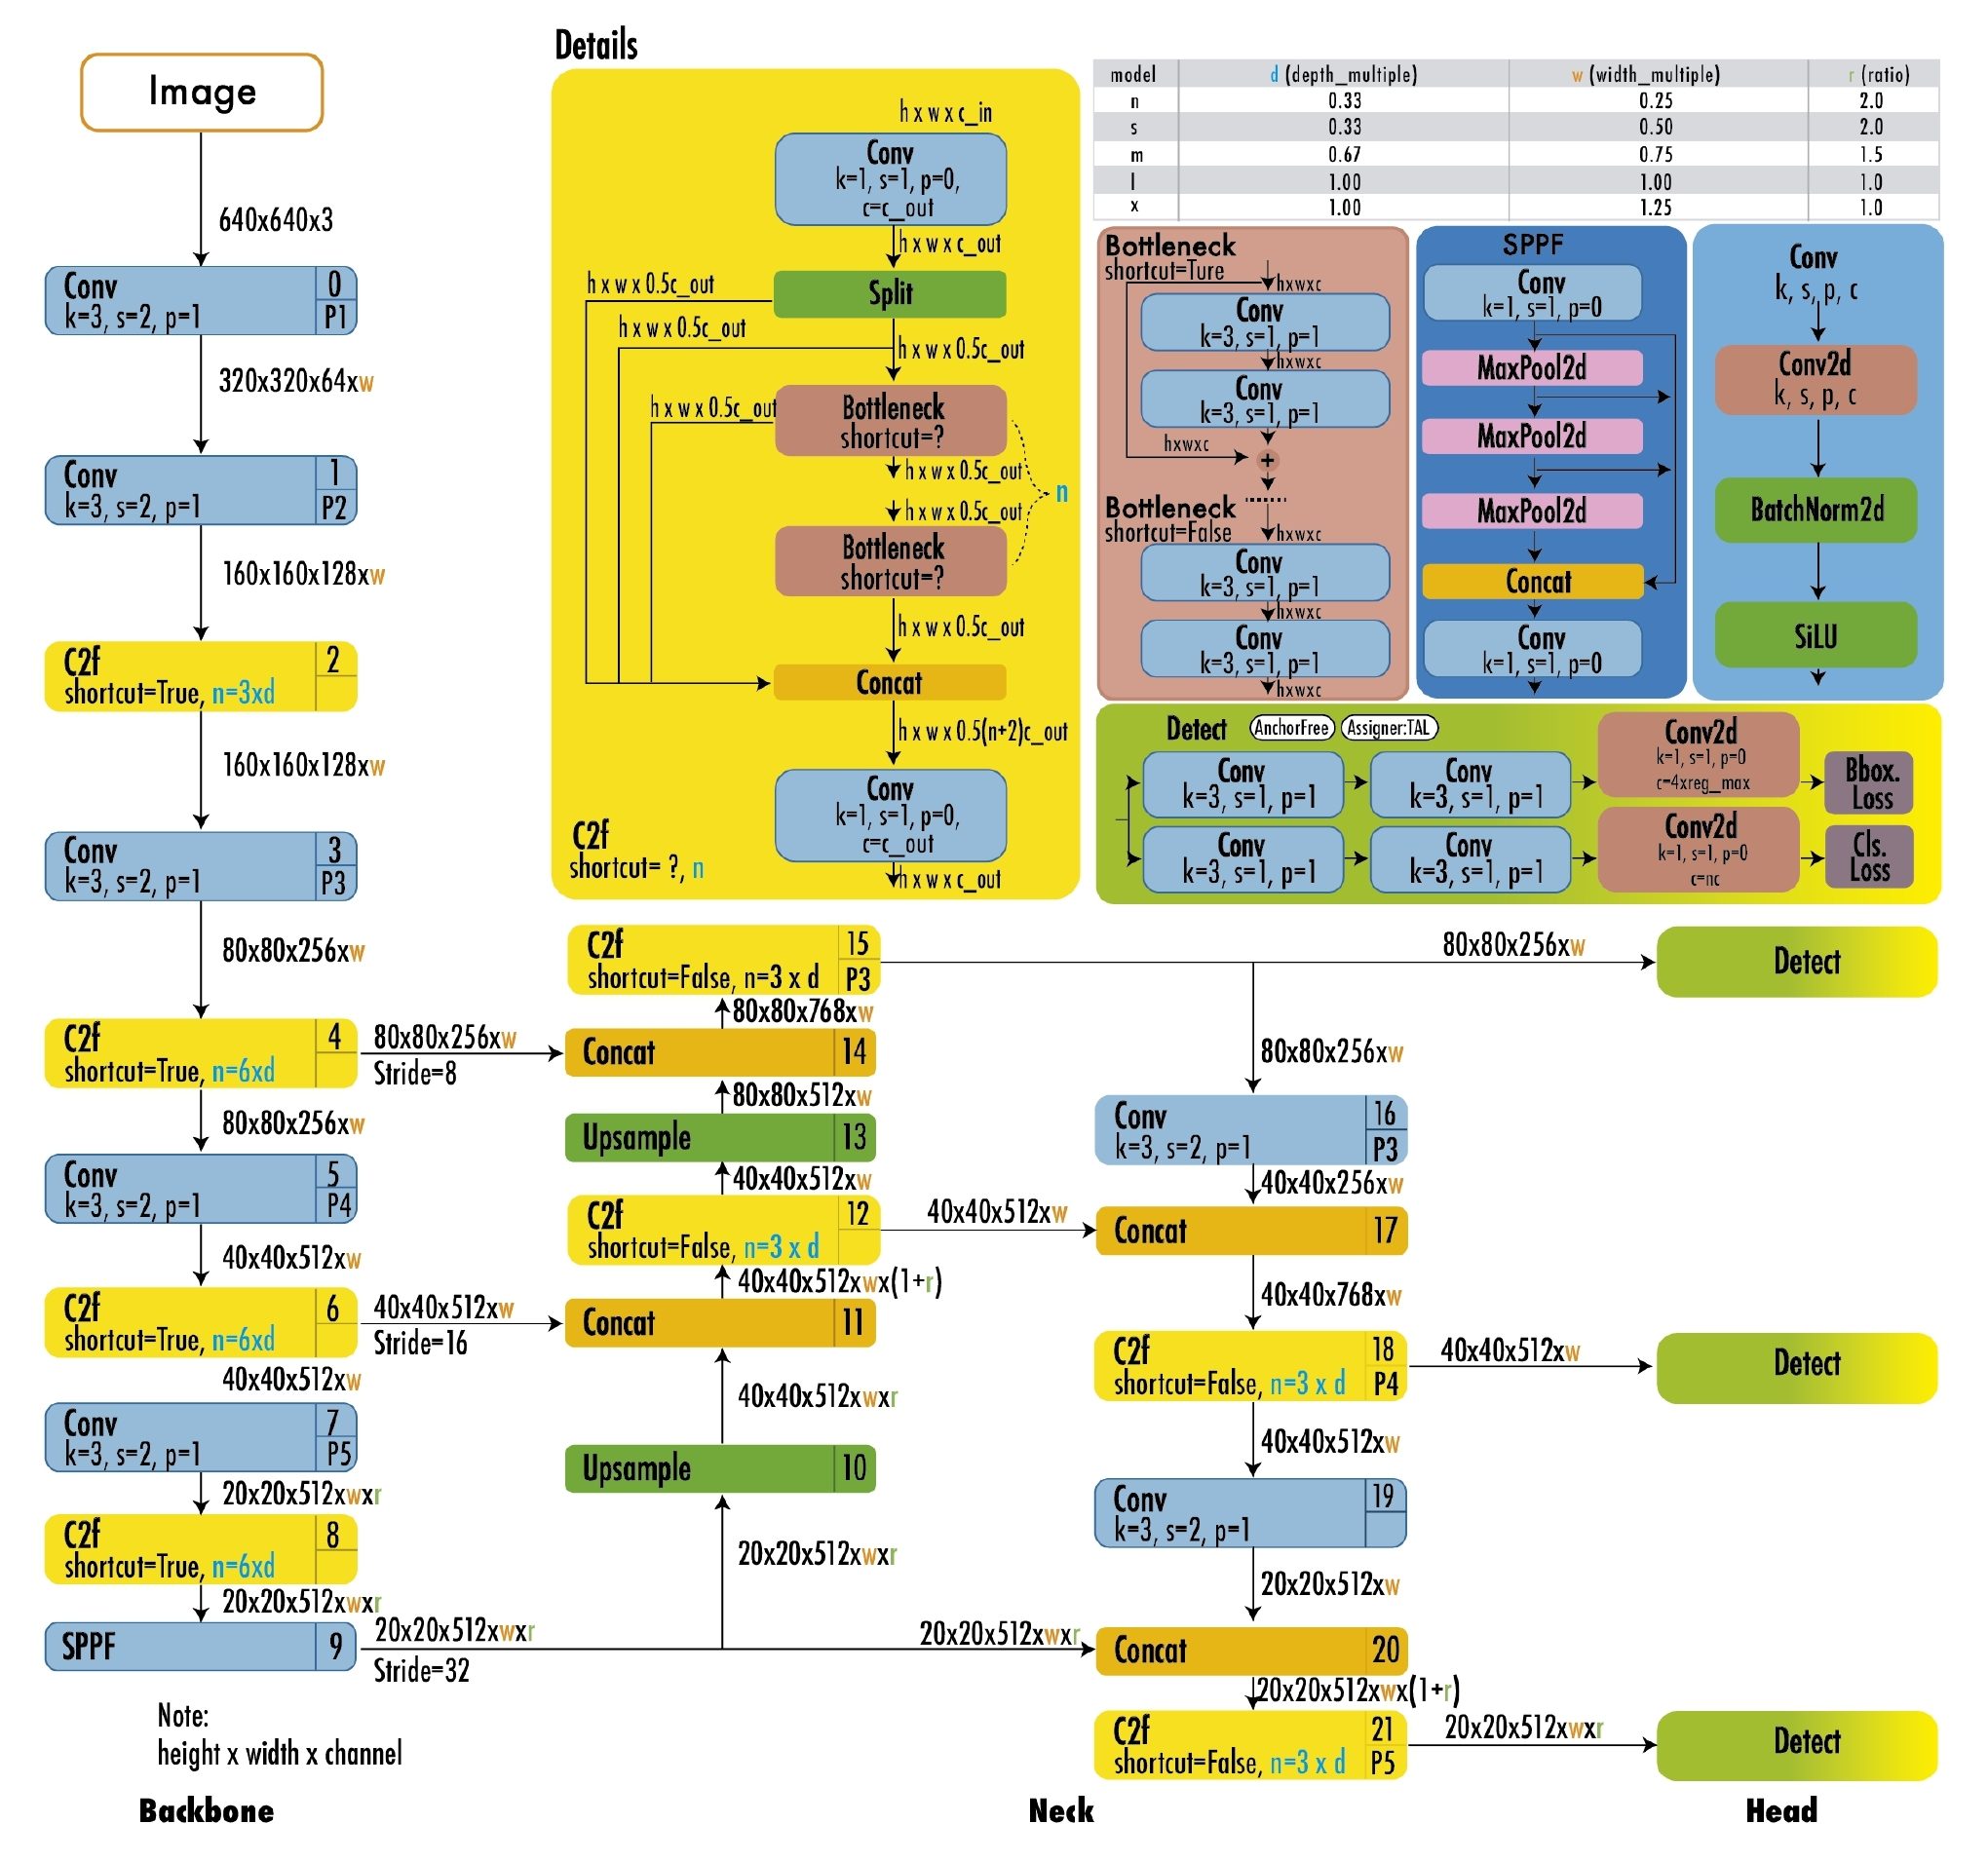
\includegraphics[scale=0.5]{images/YoloV8Architecture.jpg} 
  \caption{YOLOv8 Architecture.} 
  \label{fig:YOLOv8Architecture} 
\end{figure}

The figure shows the complete architecture of \emph{YOLOv8}, starting from the input image with a resolution of 640x640x3, which is processed through a series of convolutional layers in the \emph{Backbone} to extract important features. These features are then passed through the \emph{Neck}, which combines and processes information from various resolution levels, producing a rich multi-scale representation. Finally, the \emph{Head} is responsible for making the final predictions, such as bounding boxes, class labels, and confidence scores.

\emph{YOLOv8} predicts bounding boxes using a combination of center coordinates \((bx, by)\), bounding box dimensions \((bw, bh)\), and confidence score \(p_c\). The formula for calculating the bounding box coordinates based on the network output is:

\begin{equation}
  \begin{array}{c}
  bx = \sigma(t_x) + c_x\\
  bw = p_w e^{t_w}\\
  by = \sigma(t_y) + c_y\\ 
  bh = p_h e^{t_h}
  \end{array}
\end{equation}

Where \(t_x, t_y, t_w, t_h\) are the outputs of the neural network model, \(\sigma\) is the sigmoid function, \(c_x, c_y\) are the grid cell coordinates, and \(p_w, p_h\) are the anchor box scales.

The loss function in \emph{YOLOv8} consists of several main components that measure the difference between the model's predictions and the ground truth, balancing the importance of coordinate predictions, confidence scores, and object classification. The formula for the loss function is:

\begin{equation}
  \begin{array}{c}
  \mathbf{Loss} = \lambda_{\mathrm{coord}} \sum_{i=0}^{S^2} \sum_{j=0}^{B} \mathbb{1}_{ij}^{\mathrm{obj}} \left[ (bx_i - \hat{bx}_i)^2 + (by_i - \hat{by}_i)^2 \right] \\[10pt]
  + \lambda_{\mathrm{coord}} \sum_{i=0}^{S^2} \sum_{j=0}^{B} \mathbb{1}_{ij}^{\mathrm{obj}} \left[ (\sqrt{bw_i} - \sqrt{\hat{bw}_i})^2 + (\sqrt{bh_i} - \sqrt{\hat{bh}_i})^2 \right] \\[10pt]
  + \sum_{i=0}^{S^2} \sum_{j=0}^{B} \mathbb{1}_{ij}^{\mathrm{obj}} (C_i - \hat{C}_i)^2 + \lambda_{\mathrm{noobj}} \sum_{i=0}^{S^2} \sum_{j=0}^{B} \mathbb{1}_{ij}^{\mathrm{noobj}} (C_i - \hat{C}_i)^2 \\[10pt]
  + \sum_{i=0}^{S^2} \mathbb{1}_{i}^{\mathrm{obj}} \sum_{c \in \mathrm{classes}} (p_i(c) - \hat{p}_i(c))^2
  \end{array}
\end{equation}

In this equation, \(S\) is the grid size, \(B\) is the number of bounding boxes per grid cell, \(\mathbb{1}_{ij}^{\mathrm{obj}}\) is an indicator that bounding box j in cell i predicts an object, and \(\lambda_{\mathrm{coord}}\) and \(\lambda_{\mathrm{noobj}}\) are hyperparameters that control the importance of each loss component.

\subsubsection{YOLOv8 Pose}
\label{subsubsec: YOLOv8 Pose}

\emph{YOLOv8 Pose} is a variant of \emph{YOLOv8} specifically designed for pose estimation tasks. By combining the speed of \emph{YOLO} with precise pose detection capabilities, \emph{YOLOv8 Pose} can detect keypoints on the human body in real-time. Each bounding box not only contains information about the location and size of the object but also the coordinates of keypoints related to human pose (e.g., shoulders, elbows, knees, etc.).

\subsubsection{YOLOv10}
\label{subsubsec:YOLOv10}

\emph{YOLOv10} is a further development of \emph{YOLOv8}, with several improvements in efficiency and object detection accuracy. Like \emph{YOLOv8}, the \emph{YOLOv10} architecture consists of \emph{Backbone}, \emph{Neck}, and \emph{Head}, but with the addition of new modules such as \emph{Path Aggregation Network} (PSA) and \emph{Improved Convolutional Block} (C2fCIB).

The \emph{YOLOv10} architecture was developed by introducing several key enhancements from the foundations of \emph{YOLOv8}. The \emph{YOLOv10 Backbone} still functions as the main feature extractor but is enhanced with the \emph{SCD} (Squeeze-and-Excitation Convolutional Downsample) and \emph{C2fCIB} modules, which allow for more efficient information propagation and redundancy reduction. The newly added \emph{PSA} (Path Aggregation Network) module in the \emph{Neck} helps combine information from various paths within the network, enriching feature representation for multi-scale detection.

\subsubsection{YOLOv11}
\label{subsubsec:YOLOv11}

\emph{YOLOv11} is the latest breakthrough in the series of real-time object detectors from Ultralytics. Building on the advancements of its predecessors, \emph{YOLOv11} introduces significant improvements to its architecture, making it a powerful and adaptive solution for various computer vision applications. Ultralytics has introduced various enhancements in object detection and deep learning architecture. The improved \emph{backbone} and \emph{neck} architectures enhance feature extraction, enabling more accurate object detection and handling of more complex tasks.

Efficiency and speed are also sharpened through a refined architecture and a more optimal training pipeline, resulting in faster processing without sacrificing accuracy and performance. \emph{YOLOv11} supports implementation on various platforms, from edge devices, cloud platforms, to systems with NVIDIA GPUs, making it flexible for use in different environments. Additionally, \emph{YOLOv11} supports a variety of tasks, including object detection, instance segmentation, image classification, pose estimation, and oriented object detection (OBB). One of the main updates in the \emph{YOLOv11} architecture is the introduction of the \emph{C3K2} module, which replaces the \emph{C2F} module in \emph{YOLOv8}, as well as the addition of the \emph{C2PSA} module after the \emph{SPPF} module to further enhance detection capabilities.

\begin{figure}[H]
  \centering
  \resizebox{1\linewidth}{!}{
    \input{images/tex/architecture-yolov11.tex}
  }
  \caption{YOLOv11 Architecture}
  \label{fig:YOLOv11Architecture}
\end{figure}

The \emph{C3K2} architecture is a modified version of the \emph{C2F} module. The main difference lies in the \emph{c3k} parameter configuration. When \emph{c3k} is set to \texttt{False}, the \emph{C3K2} module behaves like the \emph{C2F} module, using the standard bottleneck structure. Conversely, when \emph{c3k} is set to \texttt{True}, the bottleneck module is replaced by the \emph{C3} module. This change can be seen in the following figure.

\begin{figure}[H]
  \centering
  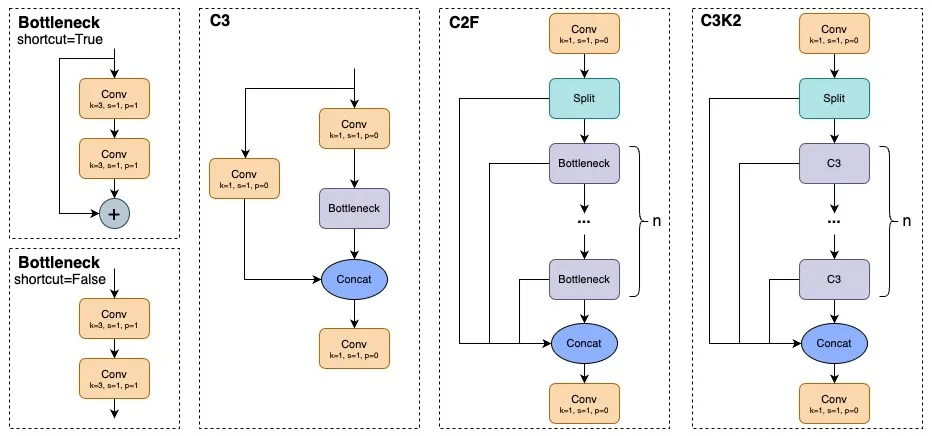
\includegraphics[scale=0.35]{images/C3k2.jpg}
  \caption{Bottleneck, C3, C2F, and C3K2 Modules}
  \label{fig:c3k2}
\end{figure}

The input features are transformed in the feedforward layer into a higher-dimensional space, allowing complex non-linear relationships to be captured more stably.

\subsection{MediaPipe}
\label{subsec:MediaPipe}

\emph{MediaPipe} is an open-source framework developed by Google for building efficient media processing pipelines, including image and video processing. This framework provides various modules that can be utilized for applications such as face detection, hand tracking, and pose estimation.

The \emph{MediaPipe} framework uses the concept of a "graph," where each node in the graph functions as a "calculator" that performs specific tasks, such as object detection, pose tracking, or image segmentation. The configuration of these nodes can be customized through \emph{GraphConfig}, which defines the topology and functionality of the entire system.

\begin{figure}[H]
  \centering
  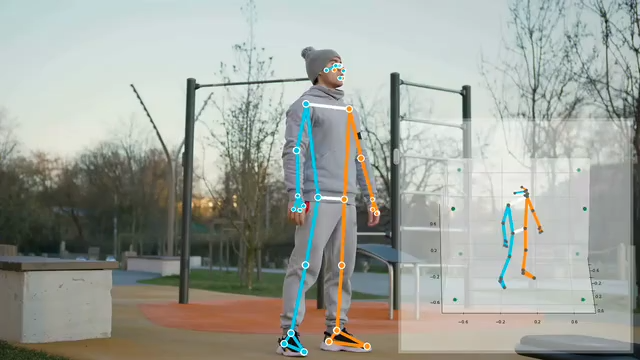
\includegraphics[scale=0.35]{images/MediaPipe3D.png}
  \caption{MediaPipe 3D}
  \label{fig:MediaPipe3D}
\end{figure}

One of the most well-known uses of \emph{MediaPipe} is human pose estimation using the \emph{MediaPipe Pose} module. This technique combines 2D pose estimation with a more complex humanoid model and uses optimization methods to calculate joint angles in 3D poses. This approach is effective in addressing depth ambiguity issues in 3D pose estimation and can work in real-time. The resulting 3D pose visualization shows each body joint as points and connecting lines between joints, providing a clear picture of the body's position and orientation in 3D space.

\subsubsection{MediaPipe Pose}
\label{subsubsec:MediaPipe Pose}

\emph{MediaPipe Pose} is a module within \emph{MediaPipe} specifically designed to detect and track human poses in real-time. Using advanced machine learning models, \emph{MediaPipe Pose} can identify up to 33 reference points on the human body, allowing the system to understand and respond to user movements quickly and accurately.

\begin{figure}[H]
  \centering
  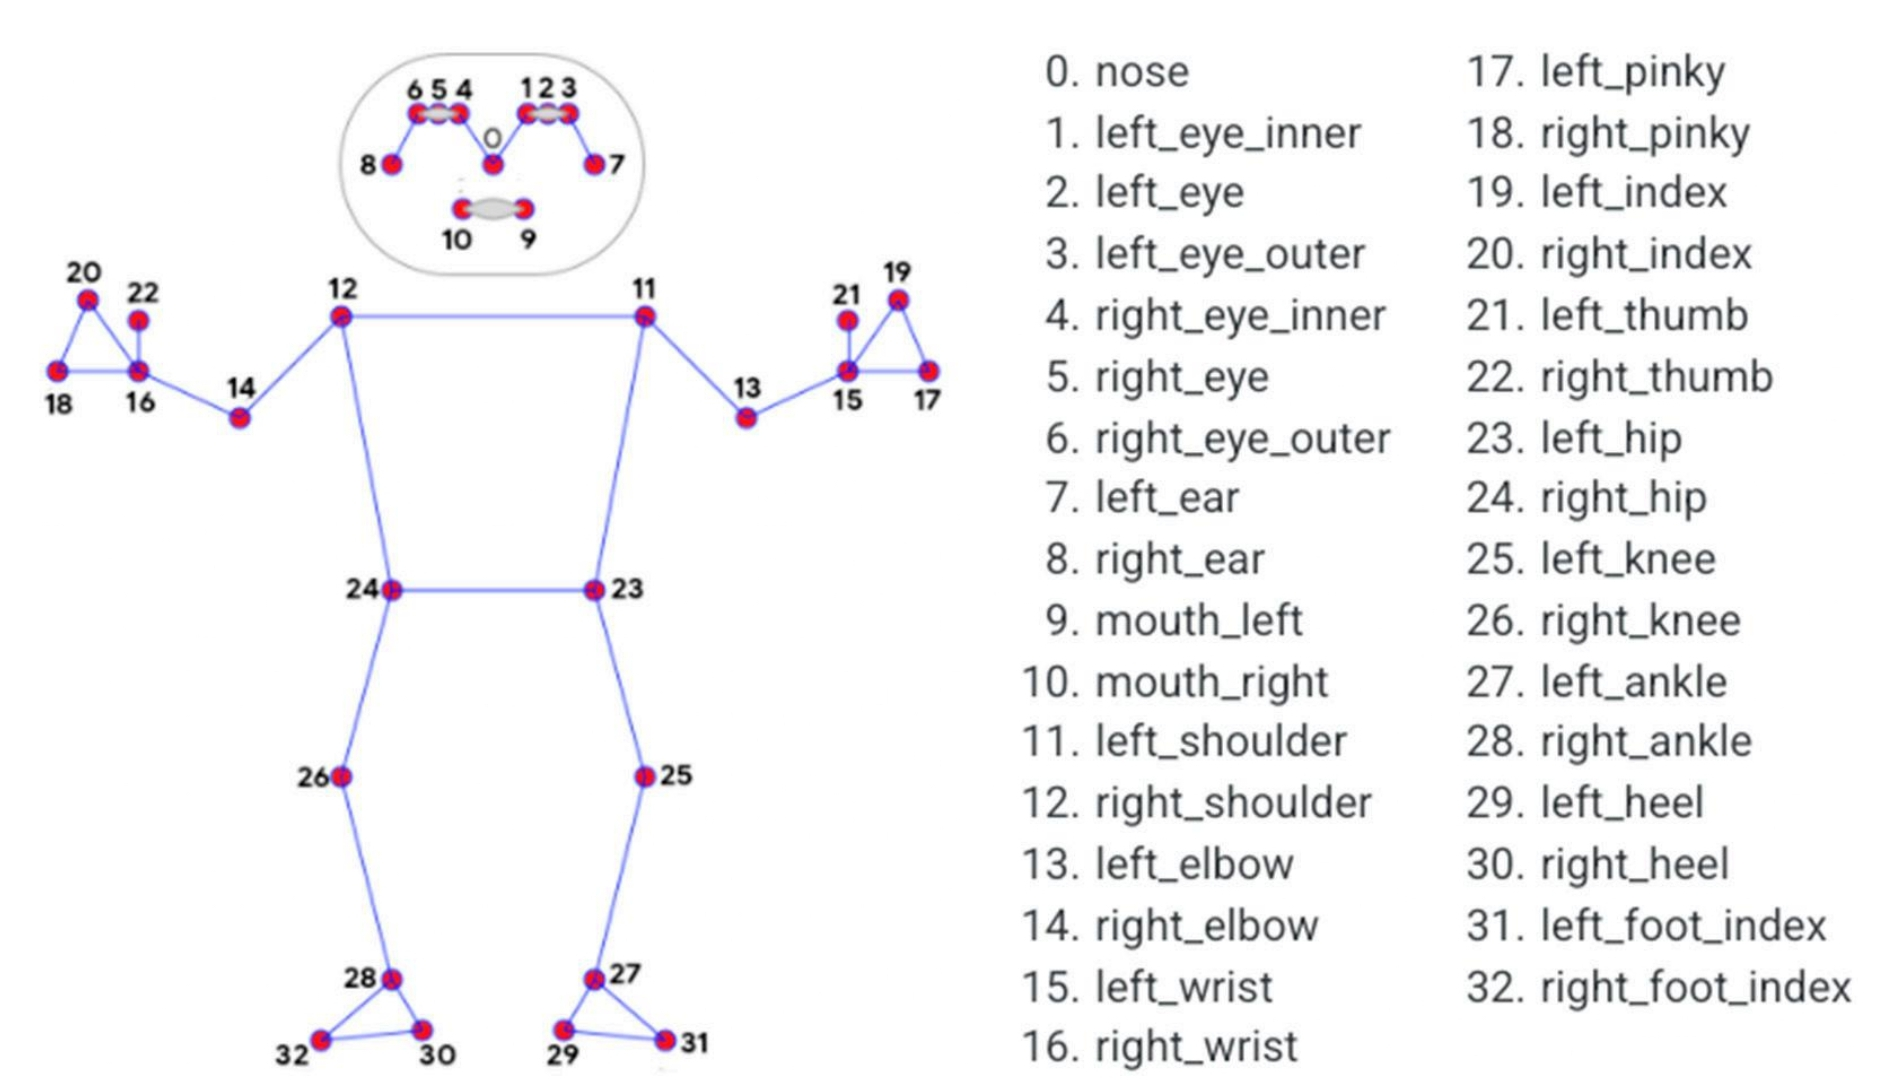
\includegraphics[scale=0.5]{images/mp_pose.jpg}
  \caption{MediaPipe Pose}
  \label{fig:mp_pose}
\end{figure}

\subsection{Classification Performance}
\label{subsec:Classification Performance}

\emph{Classification performance} refers to the ability of a model to classify input data into the correct categories. The classification process requires evaluation to assess the effectiveness of the developed model, usually using a test dataset. One commonly used evaluation approach in the context of classification is the \emph{confusion matrix}, which provides a visualization of the model's performance in categorizing data accurately.

\begin{figure}[H]
  \centering
  \includegraphics[scale=0.5]{images/ConfusionMatrix.jpg}
  \caption{Confusion Matrix.}
  \label{fig:confusion}
\end{figure}

The \emph{confusion matrix} is used to evaluate the performance of a binary classification model and displays four types of prediction results: \emph{True Positive} (TP), \emph{False Negative} (FN), \emph{False Positive} (FP), and \emph{True Negative} (TN). TP occurs when the model correctly predicts the positive class, while FN occurs when the model incorrectly predicts the negative class when it should be positive (also known as \emph{Type II Error}). FP occurs when the model incorrectly predicts the positive class when it should be negative (also known as \emph{Type I Error}), and TN occurs when the model correctly predicts the negative class.

\subsection{Evaluation Metrics}
\label{subsec:Evaluation Metrics}

Evaluation metrics serve as the basis for understanding and comparing the effectiveness of various algorithms and different scenarios. Through careful evaluation, accurate comparisons between different object detection techniques can be made, and the level of accuracy achieved can be properly assessed. This is crucial in selecting the most suitable algorithm for a specific detection task. Metrics such as \emph{accuracy}, \emph{precision}, and \emph{recall} are used to evaluate the effectiveness of a model in correctly detecting and identifying objects. Implementing these metrics is necessary to determine the most efficient model.

Additionally, accuracy analysis provides significant quantitative insights into the performance of object detection algorithms, as well as further details on the algorithm's ability to produce accurate detections. Errors identified through evaluation metrics are an important step in detection research, such as in the case of smoke detection. This identification facilitates understanding potential errors in the algorithm, which can then lead to improvements and enhancements in detection methods. Evaluation metrics are also utilized to support the optimization of algorithm hyperparameters.

In this research, various evaluation metrics such as \emph{precision}, \emph{recall}, and \emph{Mean Average Precision} (mAP) have been applied. By combining these evaluation methods, this research is designed to present a comprehensive analysis of the performance of the reviewed object detection algorithms. The explanation of the basic concepts of evaluation metrics is outlined as follows:

\subsubsection{Precision}
\label{subsubsec:precision}

\emph{Precision} is one of the main metrics used to measure how accurately the model's predictions match the detected objects. This metric indicates the proportion of true positive predictions (\emph{True Positive}) compared to the total positive predictions, both true (\emph{True Positive}) and false (\emph{False Positive}), expressed by the following equation:
\begin{equation}
  \mathrm{Precision} = \frac{TP}{TP + FP}
\end{equation}

Where \(TP\) (\emph{True Positive}): Correct prediction, i.e., detection of objects that match the ground truth, and \(FP\) (\emph{False Positive}): Incorrect prediction, i.e., detection of objects that do not match the ground truth.

\emph{Precision} is very useful in situations where false positive predictions need to be minimized. For example, in autonomous wheelchair applications, incorrect detection of humans can lead to dangerous actions, so \emph{precision} must be maintained at a high value.

\emph{Precision} is usually combined with other metrics, such as \emph{recall}, to provide a more complete picture of the model's performance.

\subsubsection{Recall}
\label{subsubsec:recall}

\emph{Recall} or sensitivity measures the model's ability to detect all objects present in an image or video. \emph{Recall} emphasizes how many objects that actually exist in the data (ground truth) are successfully detected by the model with the following equation:

\begin{equation}
  \mathrm{Recall} = \frac{TP}{TP + FN}
\end{equation}

Where \(TP\) (\emph{True Positive}): Correct prediction, i.e., objects that are correctly detected, and \(FN\) (\emph{False Negative}): Incorrect prediction, i.e., objects that exist but are not detected.

This metric is important when errors in failing to detect objects (\emph{false negative}) need to be minimized. In the context of developing an autonomous wheelchair, \emph{recall} is crucial because objects such as humans must always be detected to ensure the wheelchair can follow accurately.

\textbf{\emph{Precision and Recall Trade-off:}} In many cases, \emph{precision} and \emph{recall} have an inverse relationship. If the model is too conservative in making predictions, \emph{precision} will be high, but \emph{recall} will be low. Conversely, if the model is too lenient in detecting objects, \emph{recall} will be high, but \emph{precision} will decrease. Therefore, a balance between \emph{precision} and \emph{recall} is needed, which is usually expressed through other metrics such as \emph{F1-score}.

\subsubsection{Mean Average Precision (mAP)}
\label{subsubsec:mAP}

\emph{Mean Average Precision} (mAP) is a comprehensive metric used to measure the overall performance of an object detection model. \emph{mAP} is the average of the \emph{average precision} (AP) across all classes in the dataset.

\begin{equation}
  \mathrm{AP} = \int_0^1 P(r) \, dr
\end{equation}

Where \(P(r)\) is the \emph{Precision} as a function of \emph{recall} and \(dr\) is the differential of \emph{recall}.

AP is calculated by finding the area under the \emph{precision-recall} (PR) curve for each class. After calculating the AP for all classes, the average of these values gives the \emph{mAP}.

\begin{equation}
  \mathrm{mAP} = \frac{1}{N} \sum_{i=1}^{N} \mathrm{AP}_i
\end{equation}

Where \(N\) is the number of classes in the dataset and \(AP_i\) is the \emph{average precision} for the i-th class.

\emph{mAP} provides a broader view of the object detector's performance, as this metric considers both \emph{precision} and \emph{recall} simultaneously. The \emph{mAP} value will serve as a reference for evaluating the system's performance, such as detecting various objects like humans, obstacles, and the surrounding environment.

\subsubsection{Intersection over Union (IoU)}
\label{subsubsec:IoU}

\emph{Intersection over Union} (\emph{IoU}) is a metric used to evaluate the accuracy of object position detection performed by the model in image processing. The intersection area between the detection box generated by the model and the reference box, known as the \emph{Ground Truth}, is calculated to assess the model's performance. This ratio is obtained by comparing the area of overlap between the two boxes to the total area of their union. If the two boxes are treated as a single entity, \emph{IoU} provides a score indicating how accurately the model predicts the actual location of the object. The \emph{IoU} value increases as the proportion of the intersection area relative to the total union area increases.

\begin{figure}[H]
  \centering
  \includegraphics[scale=0.15]{images/IoU_bbox.jpg}
  \caption{Intersection over Union.}
  \label{fig:IoU_bbox}
\end{figure}

The performance of the object detection model is evaluated by comparing the overlapping area between the predicted bounding box and the ground truth bounding box. The \emph{IoU} value ranges from 0 to 1, where a value closer to 1 indicates a higher level of accuracy in detecting and locating objects.

During the evaluation process, the bounding box generated by the model is compared to the ground truth bounding box, which is manually determined as the actual location of the object in the image. The \emph{IoU} is calculated by dividing the area of overlap between the two bounding boxes by the total area of their union. The following equation is used to calculate the \emph{IoU} value:

\begin{equation}
  IoU = \frac{\left |A \bigcap B \right |}{\left | A \bigcup B \right |}
\end{equation}

\emph{IoU} is chosen as a measurement tool because of its ability to provide a clear assessment of how accurately the model identifies and bounds objects under various conditions, including variations in size, orientation, and context of objects in the image. A higher \emph{IoU} value indicates that the model can reliably detect and identify objects with a high level of precision.

\subsection{Literature Review on BoT-SORT}

BoT-SORT is a multi-object tracking (MOT) method developed with a tracking-by-detection approach. Essentially, this method leverages several techniques from previous algorithms, particularly ByteTrack, to provide more advanced tracking. Improvements in this method aim to enhance tracking performance in both dynamic and static environments by refining several key components, which will be detailed as follows \cite{aharon2022botsortrobustassociationsmultipedestrian}:
% Change the following title and label as desired.
\section{Design and Implementation}
\label{sec:designandimplementation}

\subsection{System Description}
\label{sec:systemdescription}

At this stage, the autonomous wheelchair is developed to follow humans using the YOLOv11-based detection algorithm. The system is designed with the primary goal of enhancing the mobility of users who need assistance in moving. The system consists of hardware and software components, integrated to achieve this goal.

\vspace{5pt}
\subsubsection{System Components}
\label{subsubsec:systemcomponents}

The system consists of:

\begin{itemize}
    \item \textbf{VS Code}: Used as a development environment to run YOLOv11-related code and other analyses.
    \item \textbf{Arduino IDE}: Used to develop and upload code to the ESP32 that controls the motors and sensors.
    \item \textbf{Laptop}: Serves as the main data processing center for more complex tasks and software development.
    \item \textbf{Camera (OV5640 5MP)}: Captures real-time images of the environment and detects targets (humans) using YOLOv11.
    \item \textbf{ESP32 Devkit V1}: Acts as the main controller that manages data from the camera and controls the wheelchair's movement.
    \item \textbf{2 Motor Controllers}: Control the DC motors that drive the wheelchair.
    \item \textbf{2 DC-DC Voltage Regulators}: Regulate the voltage for electronic components to remain stable.
    \item \textbf{2 DC Motors}: Drive the wheelchair, controlled through motor drivers that receive signals from the microcontroller.
    \item \textbf{24V Battery}: Serves as the main power source for the entire system, including the microcontroller, motors, and other devices.
\end{itemize}

\vspace{5pt}
\subsubsection{System Architecture}
\label{subsubsec:systemarchitecture}

The system architecture is designed so that the camera continuously captures images, then sends the data to the ESP32 microcontroller for processing. YOLOv11 is used to detect humans and provide coordinate information of the target's position. This information is then used by the microcontroller to control the motors and direct the wheelchair to dynamically follow the target's movements.

\subsection{Hardware}
\label{subsec:hardware}

The hardware design involves the integration of several components mentioned earlier. The camera is mounted at the front of the wheelchair to obtain an optimal view of the target. The ESP32 microcontroller is placed at the bottom of the wheelchair along with the motor drivers and battery to maintain balance.

\begin{itemize}
    \item \textbf{Control Unit}: A control unit such as a computer or laptop is used as the main processing center to run YOLOv11 and MediaPipe, analyze detection results, and generate decisions in the form of instruction codes.
    \item \textbf{OV5640 Camera}: This camera is connected to the ESP32 to capture frames using a 5MP sensor.
    \item \textbf{ESP32}: This microcontroller receives data from the camera and then runs the algorithm to be processed on the computer, then sends control signals to the motor driver.
    \item \textbf{L298N Motor Driver}: This driver is used to control the speed and direction of the DC motors that drive the wheelchair.
\end{itemize}

\vspace{5pt}
\subsubsection{Camera}
\label{subsubsec:camera}

The camera used in this system is the OV5640, a CMOS (Complementary Metal-Oxide-Semiconductor) camera sensor with a resolution of 5 megapixels (MP). This sensor can capture images up to a maximum resolution of 2592x1944 pixels, providing highly detailed image results. The sensor supports real-time image and video capture, with a frame rate of up to 30 frames per second (fps) at 1080p resolution, making it ideal for applications requiring direct image processing.

In addition to its high resolution, the OV5640 is also equipped with various advanced features for automatic image processing. According to the datasheet, features such as auto white balance, auto exposure, and auto focus allow this camera to automatically adapt to changes in lighting conditions and distance, thus consistently producing high-quality images in various situations. The OV5640 also supports face detection and image scaling features, which are very useful for quickly and accurately detecting objects or human targets.

\vspace{5pt}
\subsubsection{Control Unit}
\label{subsubsec:controlunit}

The control unit in this system acts as the main data processor during testing, with specifications designed to handle high computational loads and suitable for real-time data processing.

One important aspect of the control unit in this project is the support for fast and stable WiFi communication between devices. The system relies on video data sent by the OV5640 camera through the ESP32 to the laptop for processing, and this process must occur without interruption. The provided WiFi connectivity also allows real-time data transmission with minimal latency, which is crucial for quick target detection.

The ability to maintain stable WiFi connections at greater distances from the router is also important for testing in large areas. Handling multiple devices connected simultaneously allows efficient communication between ESP32 units without performance degradation. This technology is essential to ensure that the system can continuously process video data sent by the camera and provide instructions with a quick response.

The image data obtained using the OV5640 camera will be processed through a series of image data processing steps using a pre-trained detection model. This model is trained using the YOLOv11 architecture. The model used is named Best.pt, which is the result of training to detect the Human class.

To implement the system properly, several libraries need to be installed first. These libraries include OpenCV for image processing and Ultralytics for YOLO.

\begin{lstlisting}
  pip install OpenCV
  pip install Ultralytics
  ...etc
\end{lstlisting}

\vspace{5pt}
\subsubsection{ESP32}
\label{subsubsec:ESP32}

The ESP32 will receive directional data from the human detection classification results in the form of character letters such as A, B, C, D, or E. Based on previous research, the process of receiving string data by the ESP32 from connected devices is crucial for the smooth operation of the system.

Once the data is received and stored, the string is extracted into information about direction and speed. This extraction stage is crucial to convert the string into a format that can be used by the program to control the wheelchair motors. The extracted data is then displayed to ensure that the received direction and speed match the expected values. With the direction and speed information ready, the ESP32 can send instructions to the wheelchair motors to move according to the received data. This process will continue as long as the device remains connected and data continues to flow.

To provide a clearer understanding of the instructions received from the human detection classification results, the following table presents the instruction codes used in this program:

\begin{table}[H]
\centering
\caption{Instruction Codes from Classification Results}
\begin{tabular}{|c|c|}
\hline
\textbf{Pose Classification} & \textbf{Instruction Code} \\
\hline
Left & A \\
\hline
Forward & B \\
\hline
Stop & C \\
\hline
Backward & D \\
\hline
Right & E \\
\hline
\end{tabular}
\end{table}

These instruction codes are used to direct the wheelchair motors according to the detections made by the YOLOv11 classification model. For example, if the detected direction is "Left", the instruction code 'A' will be sent to move the wheelchair to the left. Similarly, if the detected direction is "Forward", the instruction 'B' will be sent to move the wheelchair forward. The code 'C' is used to stop the wheelchair when "Stop" is detected, 'D' to move backward when "Backward" is detected, and 'E' to move to the right when "Right" is detected.

This program ensures that the ESP32 functions effectively as a server receiving data from the NUC and using it to control the wheelchair motors. With the steps described, this program is designed to run continuously without interruption, waiting for and processing data sent by connected devices.

% Change the following title and label as desired.
\section{Results and Discussion}
\label{sec:resultsanddiscussion}

% Modify the paragraphs in this section as desired.
\subsection{FPS Testing}

As shown in Table \ref{tb:FPSLaptop} on the right, the average FPS value in the laptop FPS test is 13.140. The highest FPS value is 13.23, and the lowest FPS is 13.05. Additionally, as seen in Table \ref{tb:FPSLaptop}, the average FPS value in the Intel NUC test is 6.111. The highest FPS value is 6.47, and the lowest FPS is 5.54.
\begin{table}[H]
    \centering
    \caption{FPS Comparison Results on Laptop and NUC}
    \label{tb:FPSLaptop}
    \begin{tabular}{|c|c|c|}
        \hline 
        \cellcolor[HTML]{000000}                        & \cellcolor[HTML]{C0C0C0} \textbf{Laptop}  & \cellcolor[HTML]{C0C0C0} \textbf{NUC}  \\ \hline
        \cellcolor[HTML]{C0C0C0} \textbf{Average FPS} & 13.14                                      & 6.11                                    \\ \hline
        \cellcolor[HTML]{C0C0C0} \textbf{Maximum FPS}  & 13.23                                      & 6.47                                   \\ \hline
        \cellcolor[HTML]{C0C0C0} \textbf{Minimum FPS}   & 13.05                                      & 5.54                                    \\ \hline
    \end{tabular}
\end{table}

\subsection{Response Time Testing}
Based on the above output, the system's Response Time can be calculated and will be explained in Table \ref{tb:Hasil Pengujian Response Time}. The Response Time will be tested to obtain the time required for detection with the model, classification, and transmission to the ESP32 until the wheelchair motor starts moving. This test is conducted in real-time on the NUC device, with delay calculations obtained from the start of transmission until the motor stops. The inference time calculation starts from the beginning of the prediction process until the classification result is obtained. The average delay time obtained is 0.2494 seconds from the NUC test data, and the results can be seen in the table below. The average inference time obtained is 139.4899 ms or 0.1394899 seconds.
\begin{table}[H]
    \centering
    \caption{Delay Results}
    \label{tb:Hasil Pengujian Response Time}
    \begin{tabular}{|c|c|c|}
        \hline 
        \cellcolor[HTML]{000000}                        & \cellcolor[HTML]{C0C0C0} \textbf{per second}  \\ \hline
        \cellcolor[HTML]{C0C0C0} \textbf{Average Delay} & 0.249                                                                        \\ \hline
        \cellcolor[HTML]{C0C0C0} \textbf{Maximum Delay}  & 0.379                                                                      \\ \hline
        \cellcolor[HTML]{C0C0C0} \textbf{Minimum Delay}   & 0.145                                                                      \\ \hline
    \end{tabular}
\end{table}

\begin{table}[H]
    \centering
    \caption{Inference Results}
    \label{tb:Hasil Inference}
    \begin{tabular}{|c|c|}
        \hline 
        \cellcolor[HTML]{000000}                        & \cellcolor[HTML]{C0C0C0} \textbf{per millisecond}   \\ \hline
        \cellcolor[HTML]{C0C0C0} \textbf{Average Inference} & 139.489                                                                       \\ \hline
        \cellcolor[HTML]{C0C0C0} \textbf{Maximum Inference}  & 181.100                                                                        \\ \hline
        \cellcolor[HTML]{C0C0C0} \textbf{Minimum Inference}   & 123.100                                                                       \\ \hline
    \end{tabular}
\end{table}

\subsection{Detection Distance Accuracy Testing}

This test evaluates the model's ability to generate distances based on calculations on the \emph{Bounding Box} and pose. The test compares the actual object distance with the system-generated distance on an Intel NUC against a standing human. Calibration was performed at a distance of 150 cm, chosen for pose and bounding box visibility. The resulting Focal Length is 480, with K1 and K2 values of 10.922 and 24.222, respectively. These values will be used in distance accuracy tests at 150 cm, 100 cm, and 50 cm. The test aims to evaluate the system's distance measurement capability.

The test was conducted using a measuring tape attached to the camera and extended towards the researcher to obtain the distance. The values were calculated to obtain the average \emph{difference} or discrepancy produced by the system against actual measurements. The following table summarizes the average distance differences for each test.

\begin{table}[H]
    \centering
    \caption{Summary of Detection Distance Accuracy Test Results}
    \label{tb:ringkasan_pengukuran_kesesuaian}
    \begin{tabular}{|l|l|l|l|}
    \hline
    \textit{Distance} & \textit{Yolo Bbox} & \textit{MediaPipe Shoulder} & \textit{MediaPipe Hand} \\ \hline
    150 cm & 3.2 cm & 5.06 cm & 23.8 cm \\ \hline
    100 cm & 20.8 cm & 2.2 cm & 3.53 cm \\ \hline
    50 cm & 69.8 cm & 14.8 cm & 1.93 cm \\ \hline
    \end{tabular}
\end{table}

In Table \ref{tb:ringkasan_pengukuran_kesesuaian}, it is shown that at a distance of 150 cm, the largest error is in the hand landmark with a percentage of 15.86\%, and the smallest error is in the Yolo Bbox at 2.13\%. At a distance of 100 cm, the largest error is in the Yolo Bbox with a percentage of 20.8\%, and the smallest is in the shoulder landmark with a percentage of 2.2\%. At a distance of 50 cm, the largest error is in the Yolo Bbox with a percentage of 139\%, and the smallest is in the hand landmark with a percentage of 3.86\%.
\begin{table}[H]
    \centering
    \caption{Obstacle Avoidance Success Performance Table}
    \label{tb:Agungganteng}
    \begin{tabular}{|c|c|}
    \hline
    Trial & Result                                                               \\ \hline
    1         & \cellcolor[HTML]{9AFF99}Wheelchair Successfully Avoided              \\ \hline
    2         & \cellcolor[HTML]{9AFF99}Wheelchair Successfully Avoided              \\ \hline
    3         & \cellcolor[HTML]{9AFF99}Wheelchair Successfully Avoided              \\ \hline
    4         & \cellcolor[HTML]{9AFF99}Wheelchair Successfully Avoided              \\ \hline
    5         & \cellcolor[HTML]{9AFF99}Wheelchair Successfully Avoided              \\ \hline
    6         & \cellcolor[HTML]{9AFF99}Wheelchair Successfully Avoided              \\ \hline
    7         & \cellcolor[HTML]{9AFF99}Wheelchair Successfully Avoided              \\ \hline
    8         & \cellcolor[HTML]{9AFF99}Wheelchair Successfully Avoided              \\ \hline
    9         & \cellcolor[HTML]{9AFF99}Wheelchair Successfully Avoided              \\ \hline
    10        & \cellcolor[HTML]{9AFF99}Wheelchair Successfully Avoided              \\ \hline
    11        & \cellcolor[HTML]{9AFF99}Wheelchair Successfully Avoided              \\ \hline
    12        & \cellcolor[HTML]{9AFF99}Wheelchair Successfully Avoided              \\ \hline
    13        & \cellcolor[HTML]{9AFF99}Wheelchair Successfully Avoided              \\ \hline
    14        & \cellcolor[HTML]{9AFF99}Wheelchair Successfully Avoided              \\ \hline
    15        & \cellcolor[HTML]{9AFF99}Wheelchair Successfully Avoided              \\ \hline
    16        & \cellcolor[HTML]{9AFF99}Wheelchair Successfully Avoided              \\ \hline
    17        & \cellcolor[HTML]{9AFF99}Wheelchair Successfully Avoided              \\ \hline
    18        & \cellcolor[HTML]{9AFF99}Wheelchair Successfully Avoided              \\ \hline
    19        & \cellcolor[HTML]{9AFF99}Wheelchair Successfully Avoided              \\ \hline
    20        & \cellcolor[HTML]{9AFF99}Wheelchair Successfully Avoided              \\ \hline
    21        & \cellcolor[HTML]{9AFF99}Wheelchair Successfully Avoided              \\ \hline
    22        & \cellcolor[HTML]{9AFF99}Wheelchair Successfully Avoided              \\ \hline
    23        & \cellcolor[HTML]{9AFF99}Wheelchair Successfully Avoided              \\ \hline
    24        & \cellcolor[HTML]{9AFF99}Wheelchair Successfully Avoided              \\ \hline
    25        & \cellcolor[HTML]{9AFF99}Wheelchair Successfully Avoided              \\ \hline
    26        & \cellcolor[HTML]{9AFF99}Wheelchair Successfully Avoided              \\ \hline
    27        & \cellcolor[HTML]{9AFF99}Wheelchair Successfully Avoided              \\ \hline
    28        & \cellcolor[HTML]{9AFF99}Wheelchair Successfully Avoided              \\ \hline
    29        & \cellcolor[HTML]{9AFF99}Wheelchair Successfully Avoided              \\ \hline
    30        & \cellcolor[HTML]{9AFF99}Wheelchair Successfully Avoided              \\ \hline
    \end{tabular}
    \end{table}

In Table \ref{tb:Agungganteng}, the results show that avoidance was successful 30 times. Therefore, the success rate obtained from this test is 100\%. This result demonstrates that the system is capable of detecting and avoiding humans effectively.

\subsection{Avoidance Accuracy Performance}
The distance avoidance accuracy test measures the comparison between the system-generated avoidance distance and the real-world wheelchair avoidance distance from a human. The avoidance distance is set at 100 cm or 1 meter, meaning the wheelchair must avoid at this distance if a human is detected.

\begin{table}[H]
    \centering
    \caption{Summary of Avoidance Accuracy Performance Results}
    \label{tb:agungkeren}
    \begin{tabular}{|l|l|l|}
    \hline
    \textit{Distance set} & \textit{Real Error} & \textit{System Error} \\ \hline
    100 cm & 33.1 cm & 29.3 cm\\ \hline
    \end{tabular}
\end{table}

As shown in Table \ref{tb:agungkeren}, the average real measurement error is 33.1 cm, and the average system measurement error is 29.3 cm. The results do not match the set distance of 100 cm or 1 meter and tend to decrease in accuracy.

This decrease is caused by several factors, including the camera's position shaking during testing, system delays, the laptop not being charged, limiting GPU usage, and decreased laptop performance during testing due to increased laptop heat over time, resulting in lower FPS.

\subsection{Avoidance Success Performance with Two Obstacles}

\begin{table}[H]
    \centering
    \caption{Avoidance Success Performance Table with Two Obstacles}
    \label{tb:mantapkali}
    \begin{tabular}{|c|c|}
    \hline
    Trial & Result                                                  \\ \hline
    1         & \cellcolor[HTML]{9AFF99}Wheelchair Successfully Avoided \\ \hline
    2         & \cellcolor[HTML]{9AFF99}Wheelchair Successfully Avoided \\ \hline
    3         & \cellcolor[HTML]{9AFF99}Wheelchair Successfully Avoided \\ \hline
    4         & \cellcolor[HTML]{9AFF99}Wheelchair Successfully Avoided \\ \hline
    5         & \cellcolor[HTML]{9AFF99}Wheelchair Successfully Avoided \\ \hline
    6         & \cellcolor[HTML]{9AFF99}Wheelchair Successfully Avoided \\ \hline
    7         & \cellcolor[HTML]{9AFF99}Wheelchair Successfully Avoided \\ \hline
    8         & \cellcolor[HTML]{9AFF99}Wheelchair Successfully Avoided \\ \hline
    9         & \cellcolor[HTML]{9AFF99}Wheelchair Successfully Avoided \\ \hline
    10         & \cellcolor[HTML]{9AFF99}Wheelchair Successfully Avoided \\ \hline
    \end{tabular}
    \end{table}

The results show that avoidance was successful 10 times. Therefore, the success rate obtained from this test is 100\%. This result demonstrates that the system can detect and avoid two human obstacles effectively.

\subsection{Avoidance Success Performance with Three Obstacles}
\begin{table}[H]
    \centering
    \caption{Avoidance Success Performance Table with Three Obstacles}
    \label{tb:mantapkali2}
    \begin{tabular}{|c|c|}
    \hline
    Trial & Result                                                  \\ \hline
    1         & \cellcolor[HTML]{9AFF99}Wheelchair Successfully Avoided \\ \hline
    2         & \cellcolor[HTML]{9AFF99}Wheelchair Successfully Avoided \\ \hline
    3         & \cellcolor[HTML]{9AFF99}Wheelchair Successfully Avoided \\ \hline
    4         & \cellcolor[HTML]{9AFF99}Wheelchair Successfully Avoided \\ \hline
    5         & \cellcolor[HTML]{9AFF99}Wheelchair Successfully Avoided \\ \hline
    \end{tabular}
    \end{table}

The results show that avoidance was successful 5 times. Therefore, the success rate obtained from this test is 100\%. This result demonstrates that the system can detect and avoid three human obstacles effectively.

\subsection{Avoidance Success Performance with Four Obstacles}
\begin{table}[H]
    \centering
    \caption{Avoidance Success Performance Table with Four Obstacles}
    \label{tb:mantapkali3}
    \begin{tabular}{|c|c|}
    \hline
    Trial & Result                                                  \\ \hline
    1         & \cellcolor[HTML]{9AFF99}Wheelchair Successfully Avoided \\ \hline
    2         & \cellcolor[HTML]{9AFF99}Wheelchair Successfully Avoided \\ \hline
    3         & \cellcolor[HTML]{9AFF99}Wheelchair Successfully Avoided \\ \hline
    \end{tabular}
    \end{table}

The results show that avoidance was successful 3 times. Therefore, the success rate obtained from this test is 100\%. This result demonstrates that the system can detect and avoid four human obstacles effectively.

% Change the following title and label as desired.
\section{Conclusion}
\label{sec:conclusion}

% Modify the paragraphs in this section as desired.

Based on the testing results, the following conclusions can be drawn:

\begin{enumerate}
  \item The model with the highest metrics trained with various configurations is the one with the highest mAP score at IoU 0.5 of 81.85\%. This value is sufficient for performing avoidance, as seen from the excellent avoidance performance results.
  \item The performance of the NUC in FPS testing produced a lower value compared to the author's personal laptop, with a difference of 7.029 fps.
  \item The average delay obtained in the testing was approximately 0.2494 seconds, and the average inference value obtained was 139.4899 ms or 0.1394 seconds.
  \item The results show that detection using \emph{Bounding Box} and shoulder landmarks is more accurate at longer distances (150 cm and 100 cm), while arm landmarks are more accurate at closer distances (50 cm). The best average \emph{difference} for the bounding box at 150 cm is 3.2 cm, the best average \emph{difference} for shoulder landmarks at 100 cm is 2.2 cm, and the best average \emph{difference} for arm landmarks at 50 cm is 1.93 cm.
  \item Detection performance results were satisfactory in 30 test samples, with a success rate of 100\%, indicating that the system created can avoid humans very well.

\end{enumerate}

\section{Suggestions}
\label{chap:suggestions}

For further development in future research, the following suggestions can be given:

\begin{enumerate}

  \item Increase the variety of datasets to enhance detection performance.
  \item Use a device with better performance for higher fps.
  \item Improve the detection grid performance by making more detailed adjustments for better mapping.
  \item Use a device cooler when testing in an open room to avoid performance degradation.
\end{enumerate}

% Ucapan terima kasih jika ada
% \section{Ucapan Terima Kasih}
% \label{sec:ucapanterimakasih}

% Penulis mengucapkan terima kasih kepada Kementerian Riset, Teknologi, dan Pendidikan Tinggi Republik Indonesia atas \lipsum[1]

% Menampilkan daftar pustaka dengan format IEEE
\bibliographystyle{IEEEtranN}
\bibliography{pustaka/pustaka.bib}

% Menyeimbangkan bagian akhir di kedua kolom
\balance

\end{document}